\section{B-Trees}

\subsection{Introduction}\hspace*{5mm}

    B-tree are self balanced search trees designed to work well on disks.

\subsection{Definition of B-trees}

    \begin{enumerate}
        \item Every node x has the following attributes:
        \begin{enumerate}
            \item x.n: the number of keys currently stored in node x.
            \item x.n keys: $x.key_1\leq x.key_2... \leq x.key_n$
            \item x.leaf: a boolean value that indicates whether the node is a leaf
            of internal node.
        \end{enumerate}
        \item Internal node has  x.n+1 pointers to its children:
        $x.c_1,x.c_2,...x.c_{n+1}$
        \item The keys $x.key_i$ separate the ranges of keys stored in each subtree:
        if $k_i$ is any key stored in the substree with root $x.c_i$, then
        \begin{equation}
            k_1 \leq x.key_1 \leq k_2 \leq ... \leq x.key_{x.n} \leq k_{x.n+1}
        \end{equation}
        \item All leaves have the same depth, which is the tree's height h.
        \item Nodes have lower and upper bounds on the number of keys they can contain.
        We express these bounds in terms of a fixed integer $t\geq 2$ called the minimum
        degree of the B-tree
        \begin{enumerate}
            \item Every node other than the root must have at least t-1 keys. Every 
            internal node other than the root thus has at least t children. If the 
            tree is nonempty, the root must have at least 1 key.
            \item Every node may contain at most 2t-1 keys. Therefore, an internal
            node may have at most 2t children. We say that a node is full if it 
            contains exactly 2t-1 keys.
        \end{enumerate}
    \end{enumerate}

    Simplest B-tree occurs when t=2, since t=2. The node can have 1-3 keys within a 
    single node. Therefore, every internal node can have 2, 3, or 4 children. Thus 
    it is call 2-3-4 Tree.

\subsubsection{The height of a B-tree}\hspace*{5mm}

    The number of disk accesses required for most operations on B-tree
    is proportional to the height of the B-Tree.

    \textbf{Theorem:}

    If $n\geq 1$, then for any n-key B-tree T of height h and minimum degree $t\geq 2$,

    \begin{equation*}
        h \leq log_t \frac{n+1}{2}
    \end{equation*}

    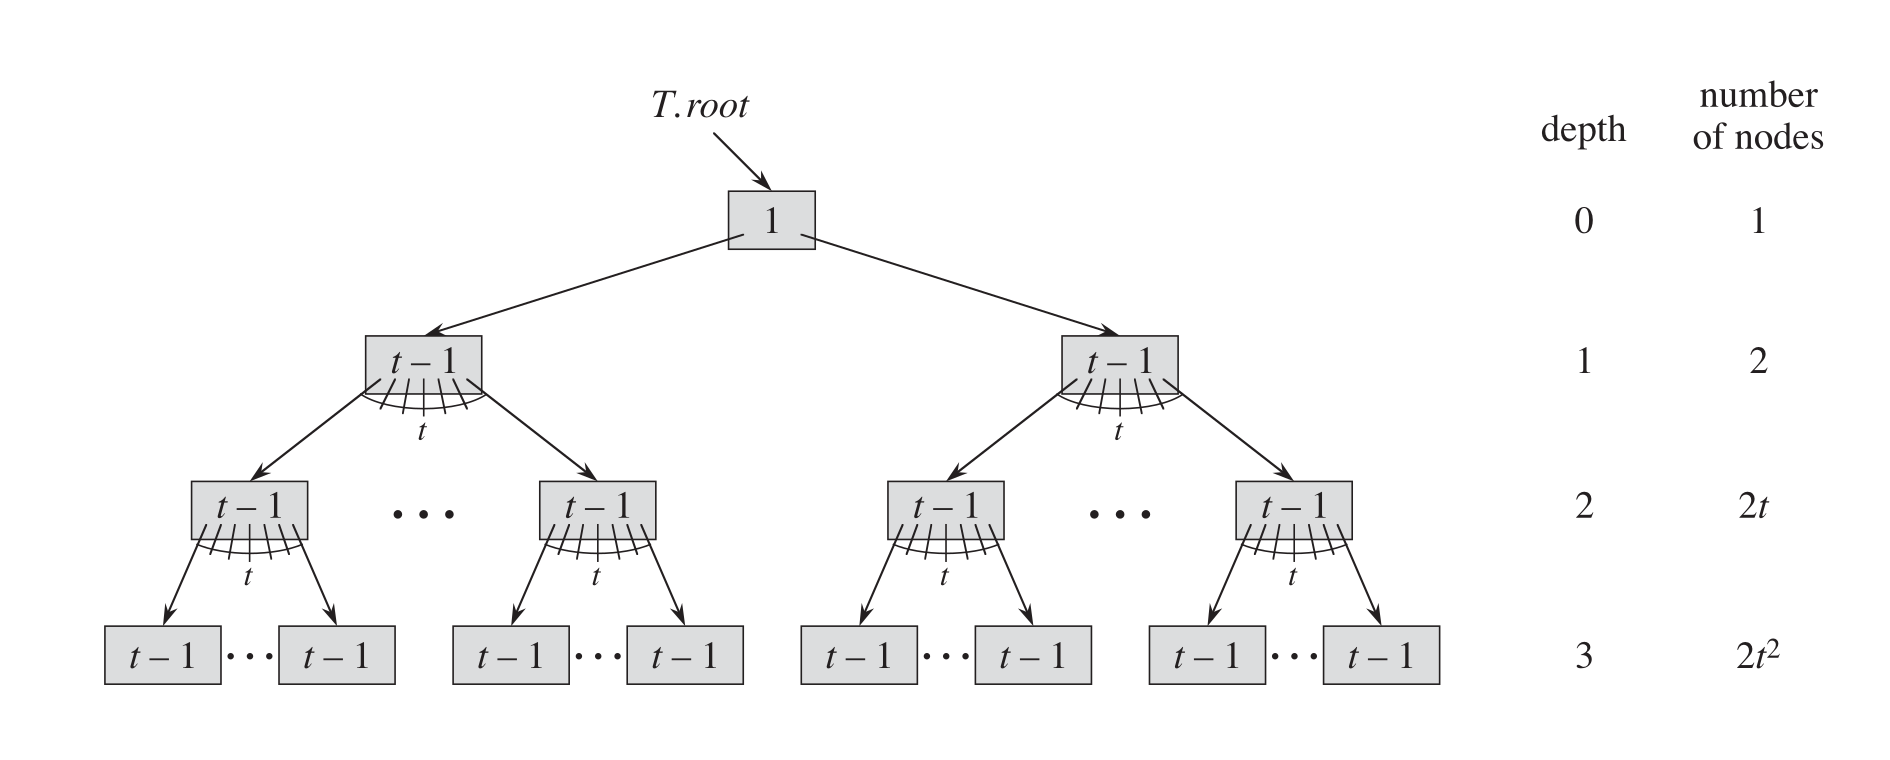
\includegraphics[width=0.7\textwidth]{contents/Advanced_Data_Structure/B_Tree/Images/B_Tree_Height.png}

    \begin{align*}
        n   &\geq 1 + (t-1)\sum_{i=1}^h 2t^{i-1}\\
            &= 1 + 2(t-1)\frac{t^h-1}{t-1}\\
            &=2t^h-1
    \end{align*}

\subsection{Create, Search and Insert}\hspace*{5mm}

    Two convention:
    \begin{enumerate}
        \item The root is always in the main memory; no DISK-READ(root), but can 
        have DISK-WRITE(root).
        \item All nodes passed as parameters must already have been DISK-READ.
    \end{enumerate}

\sssc{Search}

    \begin{lstlisting}
        B-TREE-SEARCH(x,k){
            i = 1;

            // find the smallest index i such that k <= x.key_i
            while(i <= n && k > x.key_i){
                i = i + 1;
            }
            
            // key is found in this level
            if(i<=x.n && k==x.key_i){
                return (x,i);
            }

            //reached to the leaf, and still not found
            else if(x.leaf){
                return NIL;
            }

            else{
                // bring the next node into the main memory
                DISK-READ(x.c_i)
                // search in the sandwitched child
                return B-TREE-SEARCH(x.c_i,k);
            }
        }
    \end{lstlisting}

    \textbf{\underline{Time Complexity:}}

    Within each node, there is a linear search that would takes up to 2t-1 operations.
    There would be potiential $O(h) = O(log_t n)$ calls to reach the leaf. Thus 
    a total CPU time:$O(th) = O(tlog_t n)$.

    Although, we perform $O(h) = O(log_t n)$ disk operations.

\sssc{Create}

    To create a B-tree, we need to allocate the root in the memory, and write 
    the root into the disk.

    \begin{lstlisting}
        B-TREE-CREATE(T){
            x = ALLOCATE-NODE()
            x.leaf = True
            x.n = 0
            DISK-WRITE(X)
            T.root = x
        }
    \end{lstlisting}

    \textbf{\underline{Time Complexity:}}
    The total would be O(1) disk operation, O(1) CPU usage.

\sssc{Split}

    Assume, x is a nonfull node and its child $x.c_i$ is full node that both in the 
    main memory. We could split the $x.c_i$ by the median and insert the median 
    into x. 

    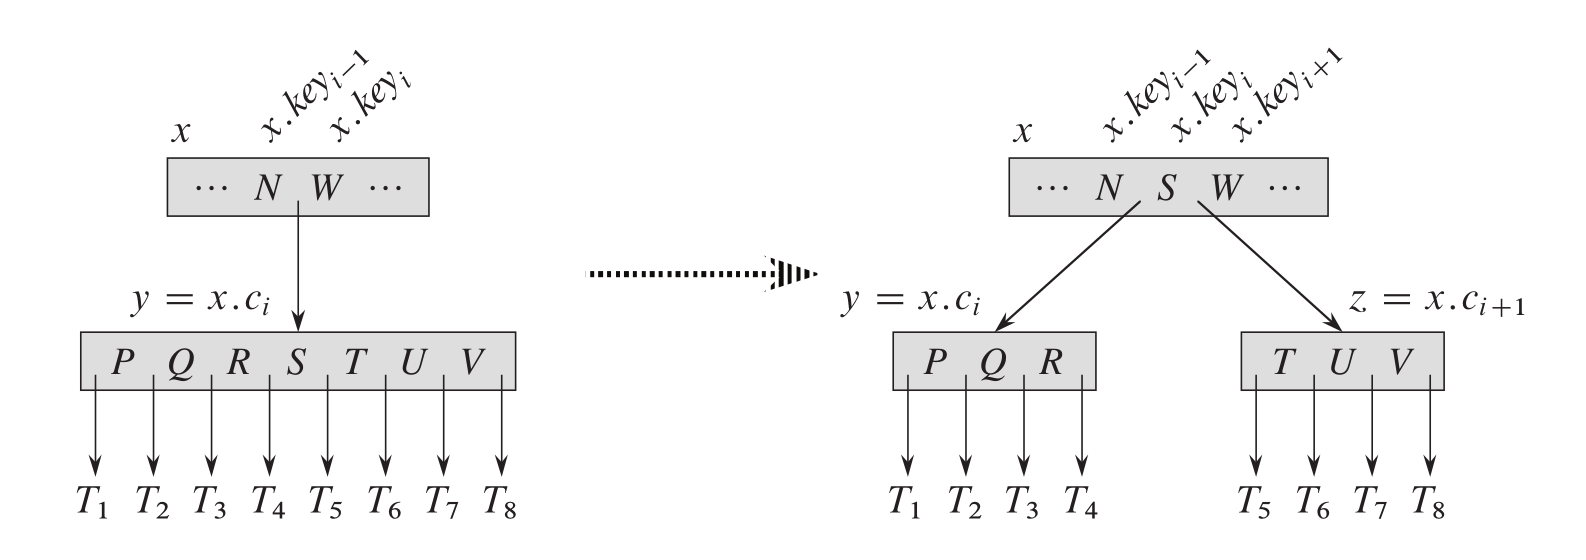
\includegraphics[width=0.6\textwidth]{contents/Advanced_Data_Structure/B_Tree/Images/B_tree_splitr.png}

    \begin{lstlisting}
        // x is the parent, i is the place of the spliting child
        B-TREE-SPLIT-CHILD(x,i){
            // allocate the space for the resulting new half
            z = ALLOCATE-NODE();
            y = x.c[i];
            
            // clone the leaf property for new half
            z.leaf = y.leaf;
            z.n = t-1;

            // both y and z would have t-1 keys
            // take away y's keys
            for(j=1 to t-1){
                z.key[j] = y.key[j+t]
            }

            // take away the y's children
            if(!y.leaf){
                for(j=1 to t){
                    z.c[j] = y.c[j+t]
                }
            }

            // set the number of keys in y
            y.n = t-1;

            // shift children one place right
            for(j=x.n+1 downto i+1){
                x.c[j+1] = x.c[j]
            }

            // attach the new half to the parent
            x.c[i+1] = z

            // shift the keys a position right 
            for(j=x.n downto i){
                x.key[j+1] = x.key[j]
            }

            // insert the median into the parent
            x.key[i] = y.key[t]
            x.n = x.n+1

            // write back to the disk to make it effect
            DISK-WRITE(y)
            DISK-WRITE(z)
            DISK-WRITE(x)

        }
    \end{lstlisting}

    \textbf{\underline{Time Complexity}}:

    The CPU time would be O(t). And O(1) disk operations.

\sssc{Insert}
    
    It would be smart to split along the searching insertion place 
    and insert in one pass.

    \begin{lstlisting}
        // T would be the B-tree, and k would be the key 
        B-TREE-INSERT(T,k){
            r = T.root
            // check whether the root is full
            if(r.n == 2t-1){
                // if it is, create a new root and allocate in the memory

                s = ALLOCATE-NODE()
                T.root = s
                s.leaf = FALSE
                s.n = 0

                // s is empty, it doesn't matter whether to attach the child
                s.c[1] = r

                // the split would add the median of orignal root into the new root
                B-TREE-SPLIT-CHILD(s,1)

                // Non root case insert
                B-TREE-INSERT-NONFULL(s,k)
            else{
                // Non root case insert
                B-TREE-INSERT-NONFULL(r,k)
            }

            }
        }
    \end{lstlisting}

        The if part would look like 

        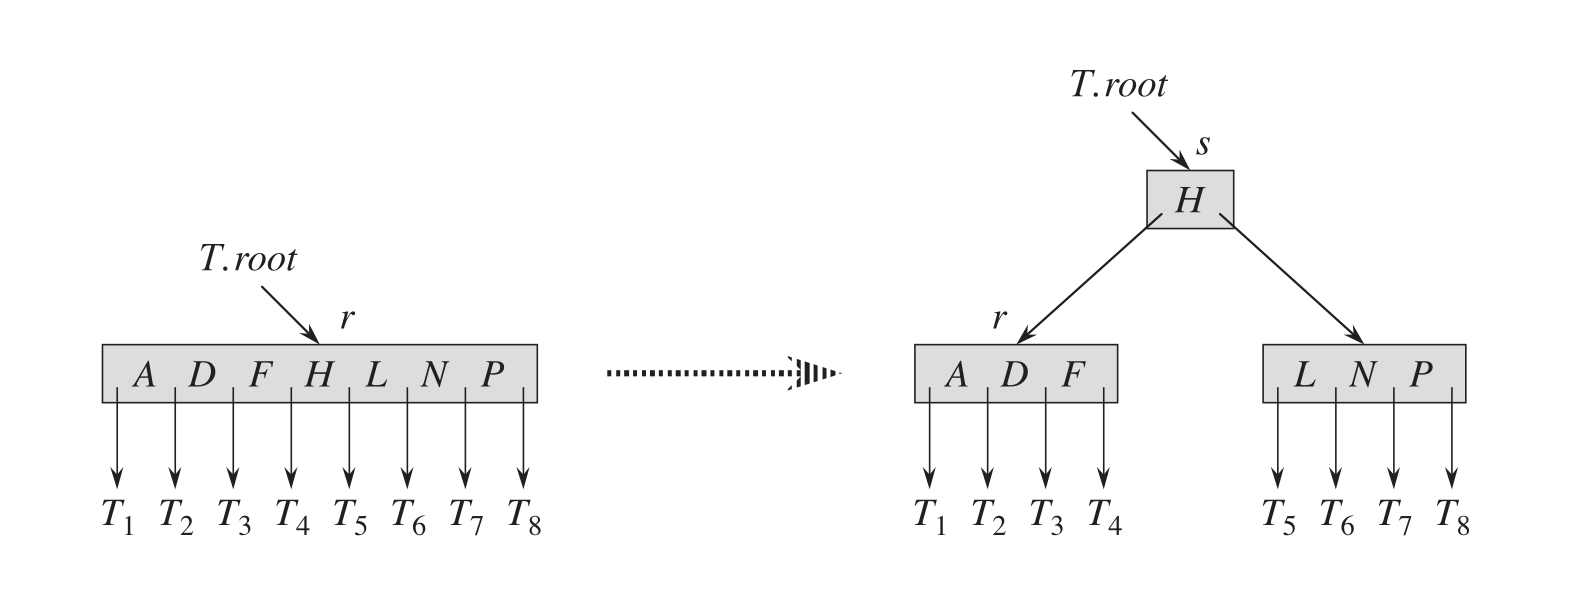
\includegraphics[width=0.65\textwidth]{contents/Advanced_Data_Structure/B_Tree/Images/split_the_root.png}

        \underline{\textbf{Note: splitting is the only way to increase the height.}}

    After spliting the root, the B-TREE-INSERT-NONFULL would inserts key k.
    The precondition of B-TREE-INSERT-NONFULL is that the given node is not full.

    \begin{lstlisting}
        // x is current node, and k is the key
        B-TREE-INSERT-NONFULL(x,k){
            i = x.n

            // leaf is the base case
            if(x.leaf){

                // shift nodes,which are greater than k, one place right
                while(i>=1 && k<x.key[i]){
                    x.key[i+1] = x.key[i]

                    // also, found the insertion position
                    i = i-1
                }

                // insert the key
                x.key[i+1] = k
                x.n = x.n+1
                
                // write back to the disk
                DISK-WRITE(x)
            }
            else{
                // found the child to be inserted into
                while(i>=1 && k<x.key[i]){
                    i = i-1
                }
                i = i+1

                // read the child into memory
                DISK-READ(x.c[i])

                // if the child is full, split
                if(x.c[i].n == 2t-1){
                    B-TREE-SPLIT-CHILD(x,i)

                    // if the key is greater than the promoted median
                    if(k > x.key[i]){
                        i = i+1
                    }
                }

                // recurse one level down
                B-TREE-INSERT-NONFULL(x.c[i],k)
            }
        }
    \end{lstlisting}


    \underline{\textbf{Time Complexity}}

    To descend to a leaf, O(h) disk operations. And the total CPU time used is
    $O(th) = O(tlog_t n)$.

\subsection{Deletion}

    The deletion is more complicated because
    \begin{enumerate}
        \item Deletion can happen in any node, not just leaf.
        \item A node(with t-1 keys) can be underflowed due to deletion.
    \end{enumerate}


    B-TREE-DELETE deletes the k from the subtree rooted at x. And whether 
    the procedure call itself recursively on node x, it is guaranteed that 
    x has at least t keys.


\sssc{Case study}


    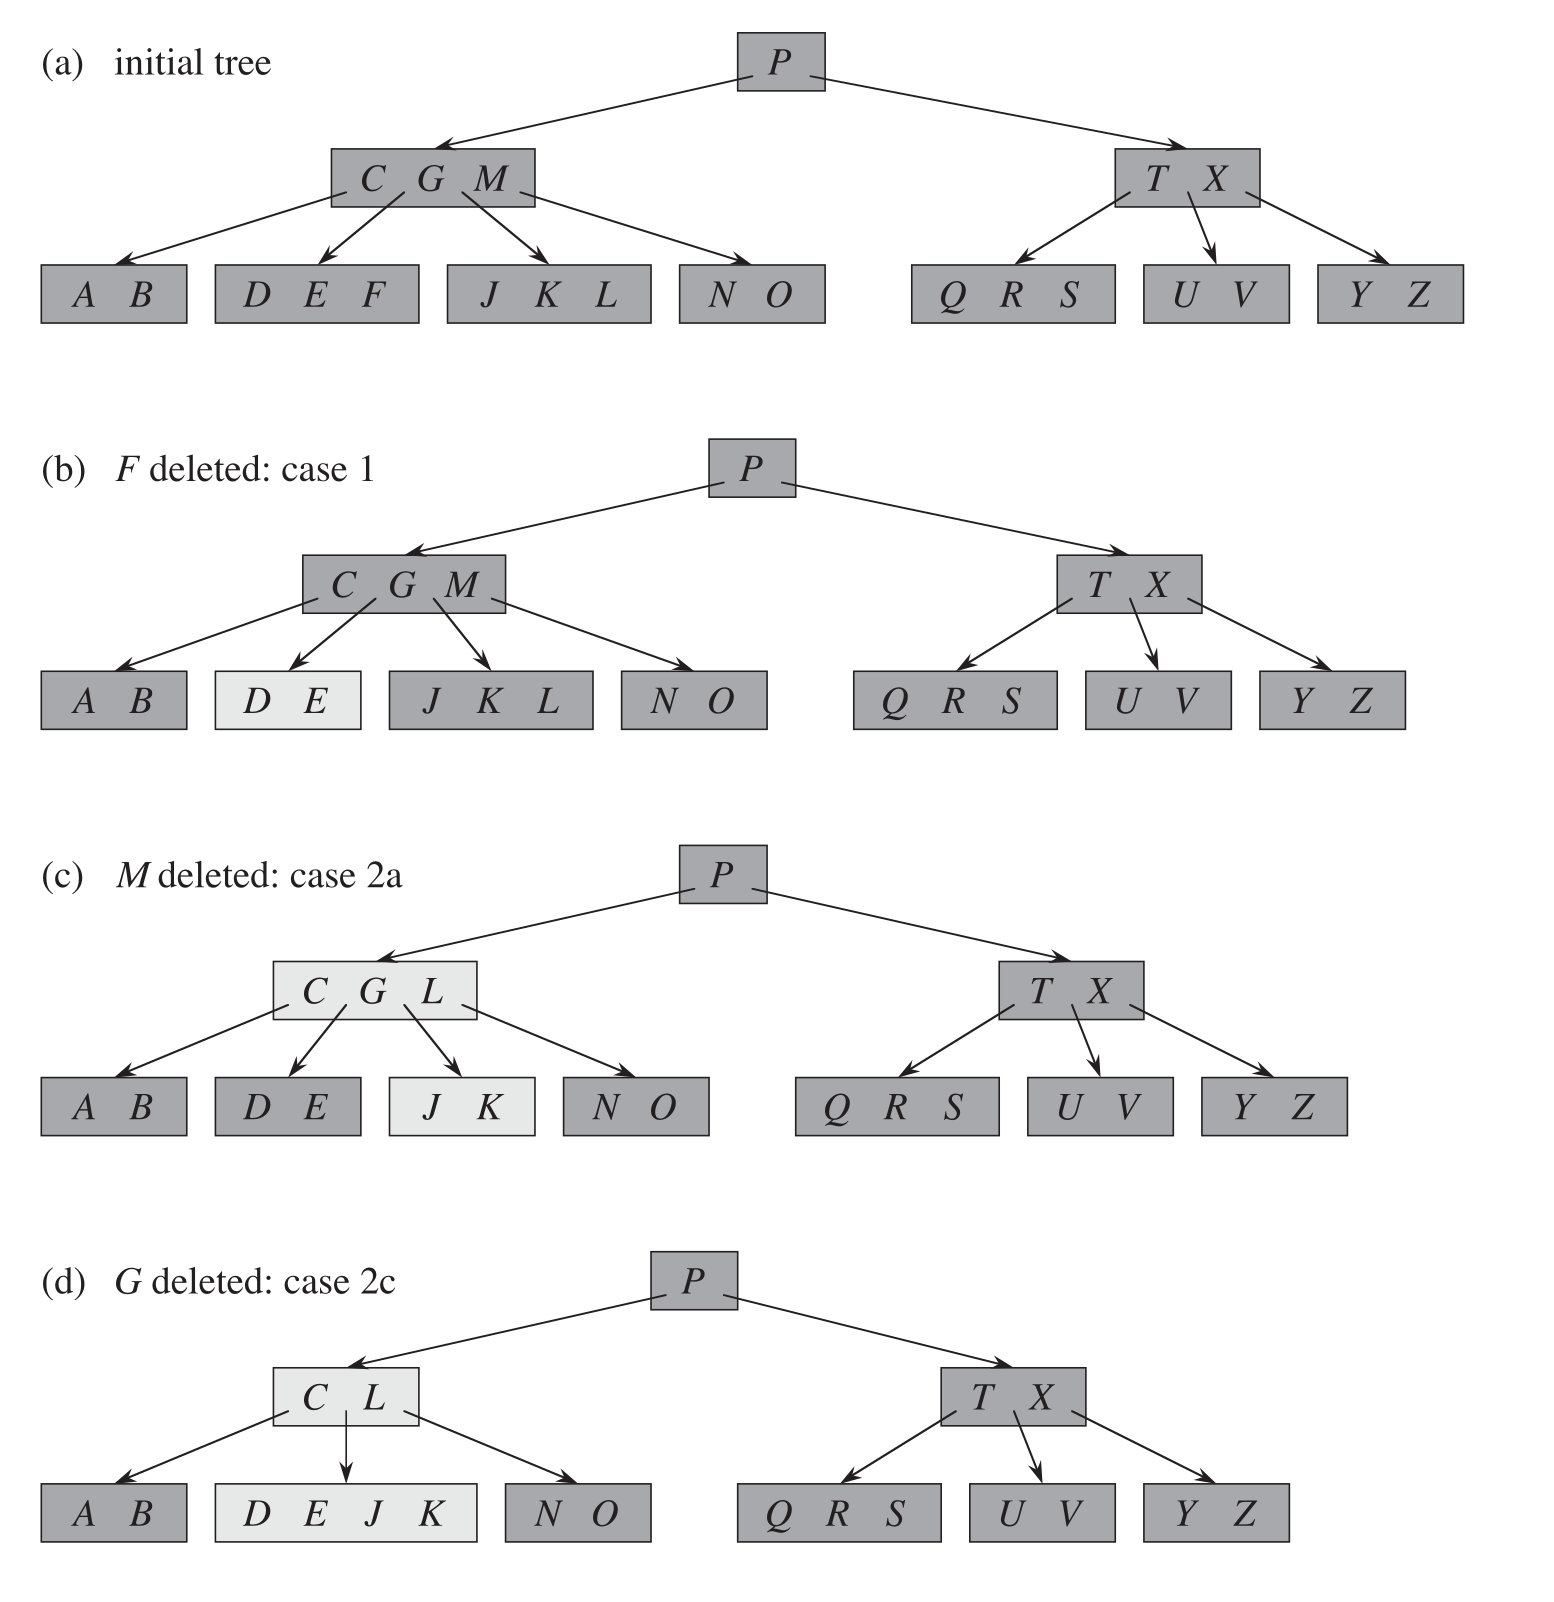
\includegraphics[width=0.7\textwidth]{contents/Advanced_Data_Structure/B_Tree/Images/case_abcd.png}

    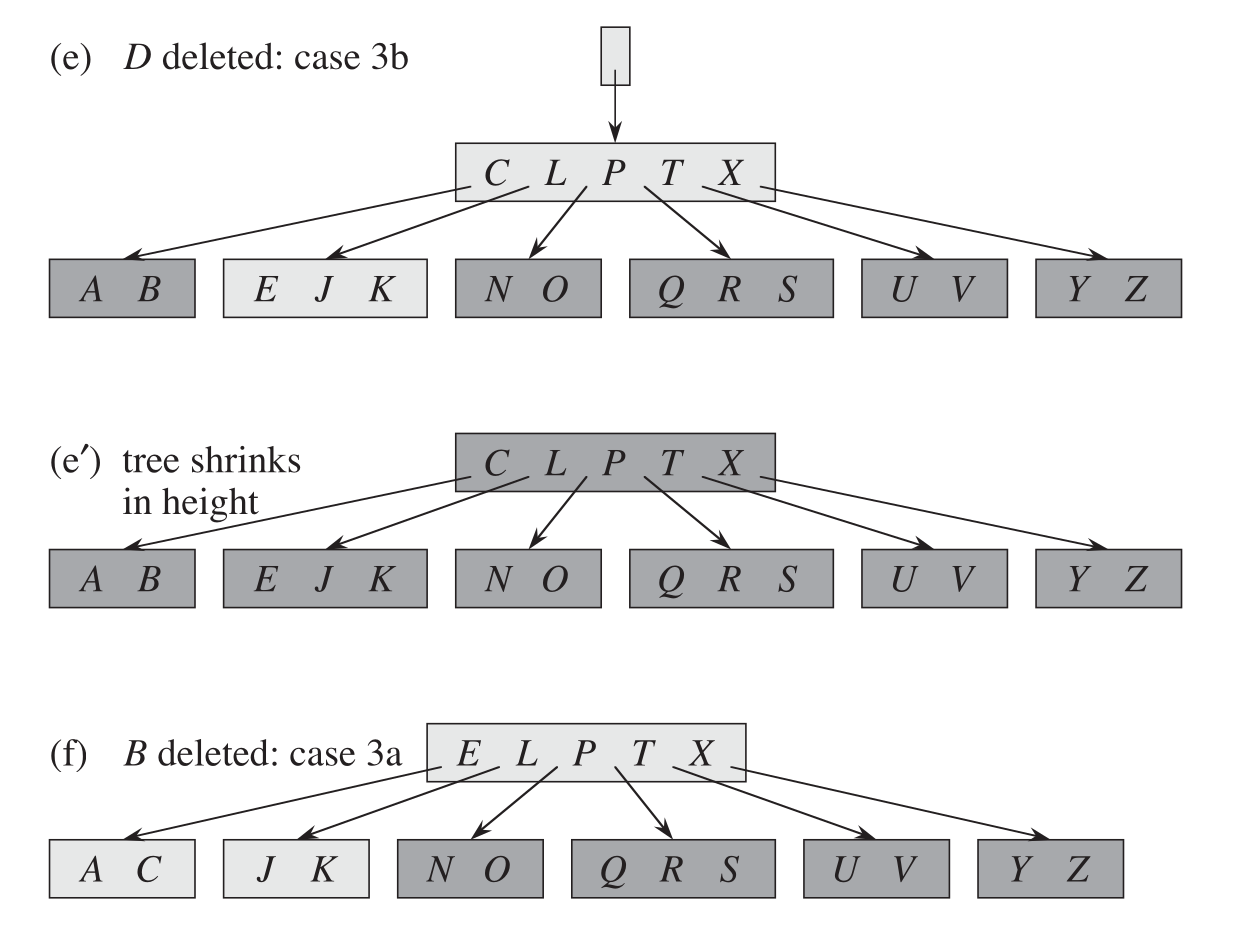
\includegraphics[width=0.7\textwidth]{contents/Advanced_Data_Structure/B_Tree/Images/deletion_ef.png}

    \begin{enumerate}
        \item If the key k is in node x and x is a leaf, delete the key from x
        \item If the key k is in node x and x is an internal node, do following
        \begin{enumerate}[label=(\alph*)]
            \item If the child y that precedes k in the node x has at least t keys,
            then find the predecessor k' of k in the substree rooted at y. Recursively 
            delete k', and replace k by k' in y.
            \item If y has fewer than t keys, then symmetrically, examine the child 
            z that follows k in the node x. If z has at least t keys, then find the 
            successor k' of k in the subtree rooted at z. Recursively delete k', and 
            replace k by k' in x.
            \item Otherwise, if both y and z have only t-1 keys, merge k and all 
            of z into y, so that x loses both k and the pointer to z, and y now 
            contains 2t-1 keys. Then free z and recursively delete k from y.
        \end{enumerate}
        \item If the key k is not present in internal node x, determine the root 
        $x.c[i]$ of subtree that contains k, if k exist. If $x.c[i]$ has only t-1 
        keys, execute 3a or 3b to make sure to descend to a node contains at least 
        t keys. Then recursively delete k from the subree that contains k.
        \begin{enumerate}[label=(\alph*)]
            \item If $x.c[i]$ has only t-1 keys but has an immediate sibling with at 
            least t keys, give $x.c[i]$ an extra key by moving a key from x down to 
            $x.c[i]$, moving a key from $x.c[i]$'s immediate sibling up to x, and 
            moving the appropriate child pointer from the sibling into $x.c[i]$.
            \item If $x.c[i]$ and both of $x.c[i]$'s immediate siblings have t-1
            keys, merge $x.c[i]$ with one sibling, which invokes moving a key from
            x down into the new merged node to become the median key for that node.
        \end{enumerate}
    \end{enumerate}
    
    \textbf{Time Complexity}:

    O(h) disk operations. CPU time required is $O(th)=O(tlog_t n)$.

    \underline{\textbf{B-TREE-DELETE is the only way to decrease the height.}}

